\chapter{BACKGROUND KNOWLEDGE}
\label{chap:background}

\paragraph{Chapter 2} Presentation of background knowledge necessary for the implementation process, including the content:

\section{Crowd-sourcing}
\subsection{Definition}
Crowdsourcing is a relatively new approach for knowledge acquisition, information diffusion, the exchange of thoughts and views among experts and the crowd, etc \cite{futureinternet0600109}. Based on this approach, several kinds of problems can be distributed and resolved through the adoption of appropriate web-based platforms designed for such a purpose. The exploitation of collective knowledge and intelligence results in the creation of innovative ideas, where in some cases, participants earn money or gain a “prize” as acknowledgment for their contribution. The advent of the World Wide Web and the spread of the Internet have led to the development of online systems through which people from all over the world have the opportunity to participate in a problem solving process with or without the contribution of experts. 

Therefore, crowdsourcing can be considered as a process evolving through the following steps: the online release of a problem, the generation of alternative solutions by the crowd (participants), the evaluation of the proposed solutions, the selection of the best provided solution and the exploitation of the selected solution by the company or institution that initially posted the problem online.

 Among the most representative crowdsourcing applications that have been developed with the upport of the so-called “crowdsourced” information are Wikipedia, Waze (a free turn-by-turn GPS application for mobile phones that uses crowdsourcing to provide routing and real-time traffic updates), Arcbazar (an American crowdsourcing platform for architectural design services), Facebook (used crowdsourcing to create different language versions of its site) and OSM (OpenStreetMap).
 
  As mentioned above, crowdsourcing is based on the principle that nobody knows everything, as everyone has a share in knowledge. In this context, the “wisdom of the crowd” can be utilized during the problem solving process through the “aggregation” of several proposed solutions \cite{doi101177}. Such a process can be facilitated by the adoption of new web technologies that offer the crucial advantage of “bringing people together”. Different views and perspectives can lead to different solutions, some of which may be unexpectedly remarkable.
  
  
  On the other hand, participants in a crowdsourcing process gain several benefits. They acquire new skills. They perceive the “seeking to the best solution” process as a challenge to achieve, and they also gain new knowledge. In some cases, they can also “incorporate that experience in the seeking of better employment or in the goal of establishing oneself in freelance work as an entrepreneur” \cite{doi101177}. Crowdsourcing is a model appropriate for the utilization of collective talents by aggregating collective intelligence and knowledge and also by increasing the ingenuity of the crowd. This may result in innovative solutions by reducing the cost and time a traditional problem solving process usually requires \cite{doi101177}

\section{MVC model}
%% chưa parapharse https://developer.mozilla.org/en-US/docs/Web/Apps/Fundamentals/Modern_web_app_architecture/MVC_architecture %%
\subsection{Definition}
Model View Controller (MVC) is a software architecture pattern, commonly used to implement user interfaces: it is therefore a popular choice for architecting web apps. In general, it separates out the application logic into three separate parts, promoting modularity and ease of collaboration and reuse. It also makes applications more flexible and welcoming to iterations.

\section{Neural network}

\subsection{Artificial Neural Network (ANN)}
The human brain consists of many computational units called neuron. The \textbf{Artificial neural network (ANN)} is vaguely inspired by that structure. An ANN is a collection of connected nodes called the artificial neurons. Each artificial neuron is a computational unit with inputs and an output. A connection between two artificial neurons is called an ‘edge’. Artificial neurons and edges will have a ‘weight’ value to adjust the learning process. Increasing or decreasing the weight value will affect the strength of the signal between two neurons. A typical artificial neuron will take each input, multiply it with the corresponding weight, take the sum of its input and apply some non-linear function to get the output. Many connections of artificial neuron form a neural network, where the output of a neuron is the input of another artificial neuron. Typically, an artificial neuron network will have many layers. If the weight is set correctly, the ANN can be used to estimate numerous complex mathematical problems.
Figure 2 represents a simple artificial neural network, where each circle is an artificial neuron, inward and outward arrows are the inputs and outputs of that neuron. The first layer where there is no input is called the “input layer”. Similarly, the last layer where there is no output is called the ‘output layer’. Layers that are either input or output are called “hidden layers”. In the figure, every neuron of one layer is connected to all neuron in the next layer, so it every layer is a “fully-connected layer”.
\begin{center}
  \begin{figure}[H]
  \centering
  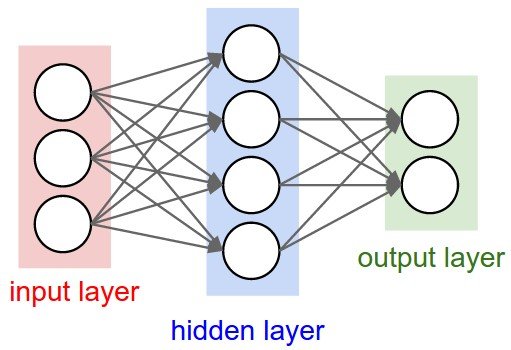
\includegraphics[width=0.75\columnwidth]{images/chap2/neural_net.png}
  \footcaption{A 2-layer Neural Network (one hidden layer of 4 neurons (or units) and one output layer with 2 neurons), and three inputs.}
  \label{chap2:neural_net}
  \end{figure}
\end{center}
\footnotetext{Source: \url:{ https://devblogs.nvidia.com/mocha-jl-deep-learning-julia/}}

\subsection{Convolution Neural Network (CNN)}

\subsection{Recurrent Neural Network (RNN)}
Human understanding does not come from scratch for every new input. When a man is reading a paragraph, his understanding of each word is based on his knowledge of previous words. That is why a human brain is persistent.\\
Traditional neural networks cannot do the task above. For example, if a traditional network wants to classify a frame in a video, it cannot use its reasoning of previous frames to help with the result of the current frame.\\
\textbf{Recurrent Neural Networks (RNN)} fix this issue by having loops within them, thus allowing information to be persistent. The remaining of this section is about the basics of RNN and \textbf{Long Short-Term Memory Network (LSTM)}, a variation of RNN designed to avoid the long-term dependencies problem of RNNs.
\subsubsection{RNN}
\textbf{Recurrent Neural Network} is a type of neural network effective for processing sequential data.
\subsubsection{LSTM}

\section{Face recognition}
\section{Action recognition}
\section{Cloud computing}
